\documentclass[a4paper]{article}

%% Language and font encodings
\usepackage[english]{babel}
\usepackage[utf8]{inputenc}
\usepackage{ragged2e}

% for figures
\usepackage{graphicx}

% for hyperlinks
\usepackage[colorlinks = true,
            linkcolor = blue,
            urlcolor  = blue,
            citecolor = blue,
            anchorcolor = blue]{hyperref}

% for pseudocode
\usepackage{algorithm}
\usepackage{algpseudocode}
% for coloring
\usepackage[usenames,dvipsnames,svgnames]{xcolor}

% bibliography
\usepackage[backend=biber,citestyle=authoryear]{biblatex}
\addbibresource{FDTD_paper.bib}

% paragraph spacing
\setlength{\parindent}{0em}
\setlength{\parskip}{0.5em}

\begin{document}

\title{Simulating electromagnetic wave propagation in ice with finite difference time domain}
\author{Ben Hills}
\maketitle

\justify
\textbf{Abstract:} Radar and seismic methods are used as geophysical techniques in many disciplines within the earth sciences. These techniques tell us something about the internal structure of a material that we can not physically see into. The utility of that knowledge is widespread. For example, geophysical methods are commonly used in the cryosphere to know the internal form of snow and ice masses, thereby giving indirect information about the accumulation and deformation of the mass

\raggedright
\section{Introduction}
Radar and seismic methods are used as geophysical techniques in many disciplines within the earth sciences. These techniques tell us something about the internal structure of a material that we can not physically see into. The utility of that knowledge is widespread. For example, geophysical methods are commonly used in the cryosphere to know the internal form of snow and ice masses, thereby giving indirect information about the accumulation and deformation of the mass
itself. 

\par
As a project for ESS 511, Geophysical Continuum Mechanics, I will simulate these equations for electromagnetic wave propagation through ice. Starting in one dimension, I will prescribe some contrasts in the material constants that force a reflection of the wave back toward the surface. Provided that I have time I will move on to a two-dimensional model. Finally, I will discuss the practical applications of this model in glaciology research \cite{Christianson2016} as well as the general use of geophysical techniques in this field.

\section{Methods}

\subsection{Maxwell's Equations}

\par
As with any physical process, using a computer model as a simulation can help us better understand the process itself. In this case, we can use Maxwell's curl equations to simulate the propagation of an electromagnetic wave through ice. Following \cite{Irving2006}, the equations are written as. 


Frequency Domain
\begin{equation}
    \nabla \times \textbf{E} = -i\omega \mu \textbf{H}
\end{equation}
\begin{equation}
    \nabla \times \textbf{H} = \sigma \textbf{E} + i\omega \epsilon \textbf{E}
\end{equation}

Time Domain
\begin{equation}
    \nabla \times \textbf{E} = - \frac{\partial B}{\partial t}
\end{equation}
\begin{equation}
    \nabla \times \textbf{H} + J =\frac{\partial D}{\partial t}
\end{equation}

Constitutive Equations

\begin{equation}
    B = \mu H    
\end{equation}
\begin{equation}
    D = \epsilon E    
\end{equation}

\subsection{Finite Difference Method}

Taylor Series

\begin{equation}
    f(x_i + \Delta x_i) = f(x_i) + \Delta x_i \left. \frac{\partial f}{\partial x} \right\vert_{x_i} + \frac{\Delta x_i^2}{2!} \left. \frac{\partial^2 f}{\partial x^2} \right\vert_{x_i} + \dots
\end{equation}

Finite Difference

\begin{equation}
    \left. \frac{\partial f}{\partial x} \right\vert_{x_i} = \frac{f(x_i + \Delta x_i) - f(x_i)}{\Delta x_i} + O(\Delta x_i)
\end{equation}


\subsection{Finite Difference Time Domain}

\subsubsection{Yee Grid}

\begin{figure}
    \centering
    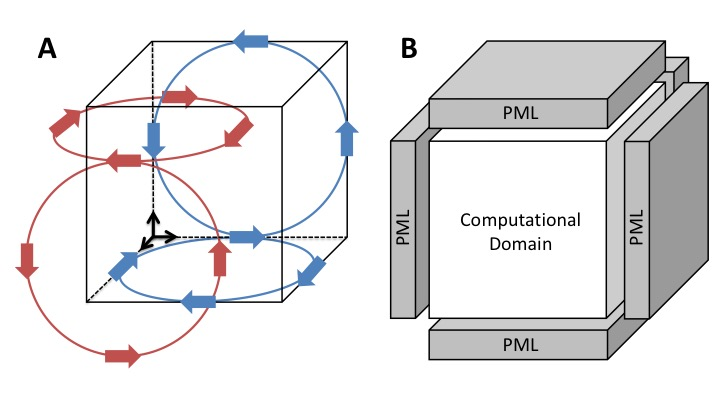
\includegraphics[width=\textwidth]{Methods_Figure.jpg}
    \caption{a) Yee Grid b) Perfectly matched layer boundary condition}
    \label{fig:YeePML}
\end{figure}

\subsubsection{PML}

\begin{center}
    \colorbox[RGB]{239,240,241}{
    \begin{minipage}{.9\linewidth}
        \begin{algorithmic}[H]
            \For{x in range(x):}
            \State H+=1
            \EndFor
        \end{algorithmic}
    \end{minipage}}
\end{center}

PML in 2 or 3 dimensions

\subsubsection{FDTD Modes}

Hx-Ey mode

\begin{equation}
    H_i^{n+1} = H_i^n + \frac{\Delta t}{\mu} \left( \frac{E_{j+1 \slash 2}^n - E_{j- 1 \slash 2}^n}{\Delta x_j} \right) 
\end{equation}

\begin{equation}
    E_i^{n+1\slash 2} = E_i^{n-1\slash 2} + \frac{\Delta t}{\epsilon} \left( \frac{H_{j+1}^n - E_{j}^n}{\Delta x_j} \right) 
\end{equation}

Ez Mode

\section{Results}

\begin{figure}
    \centering
    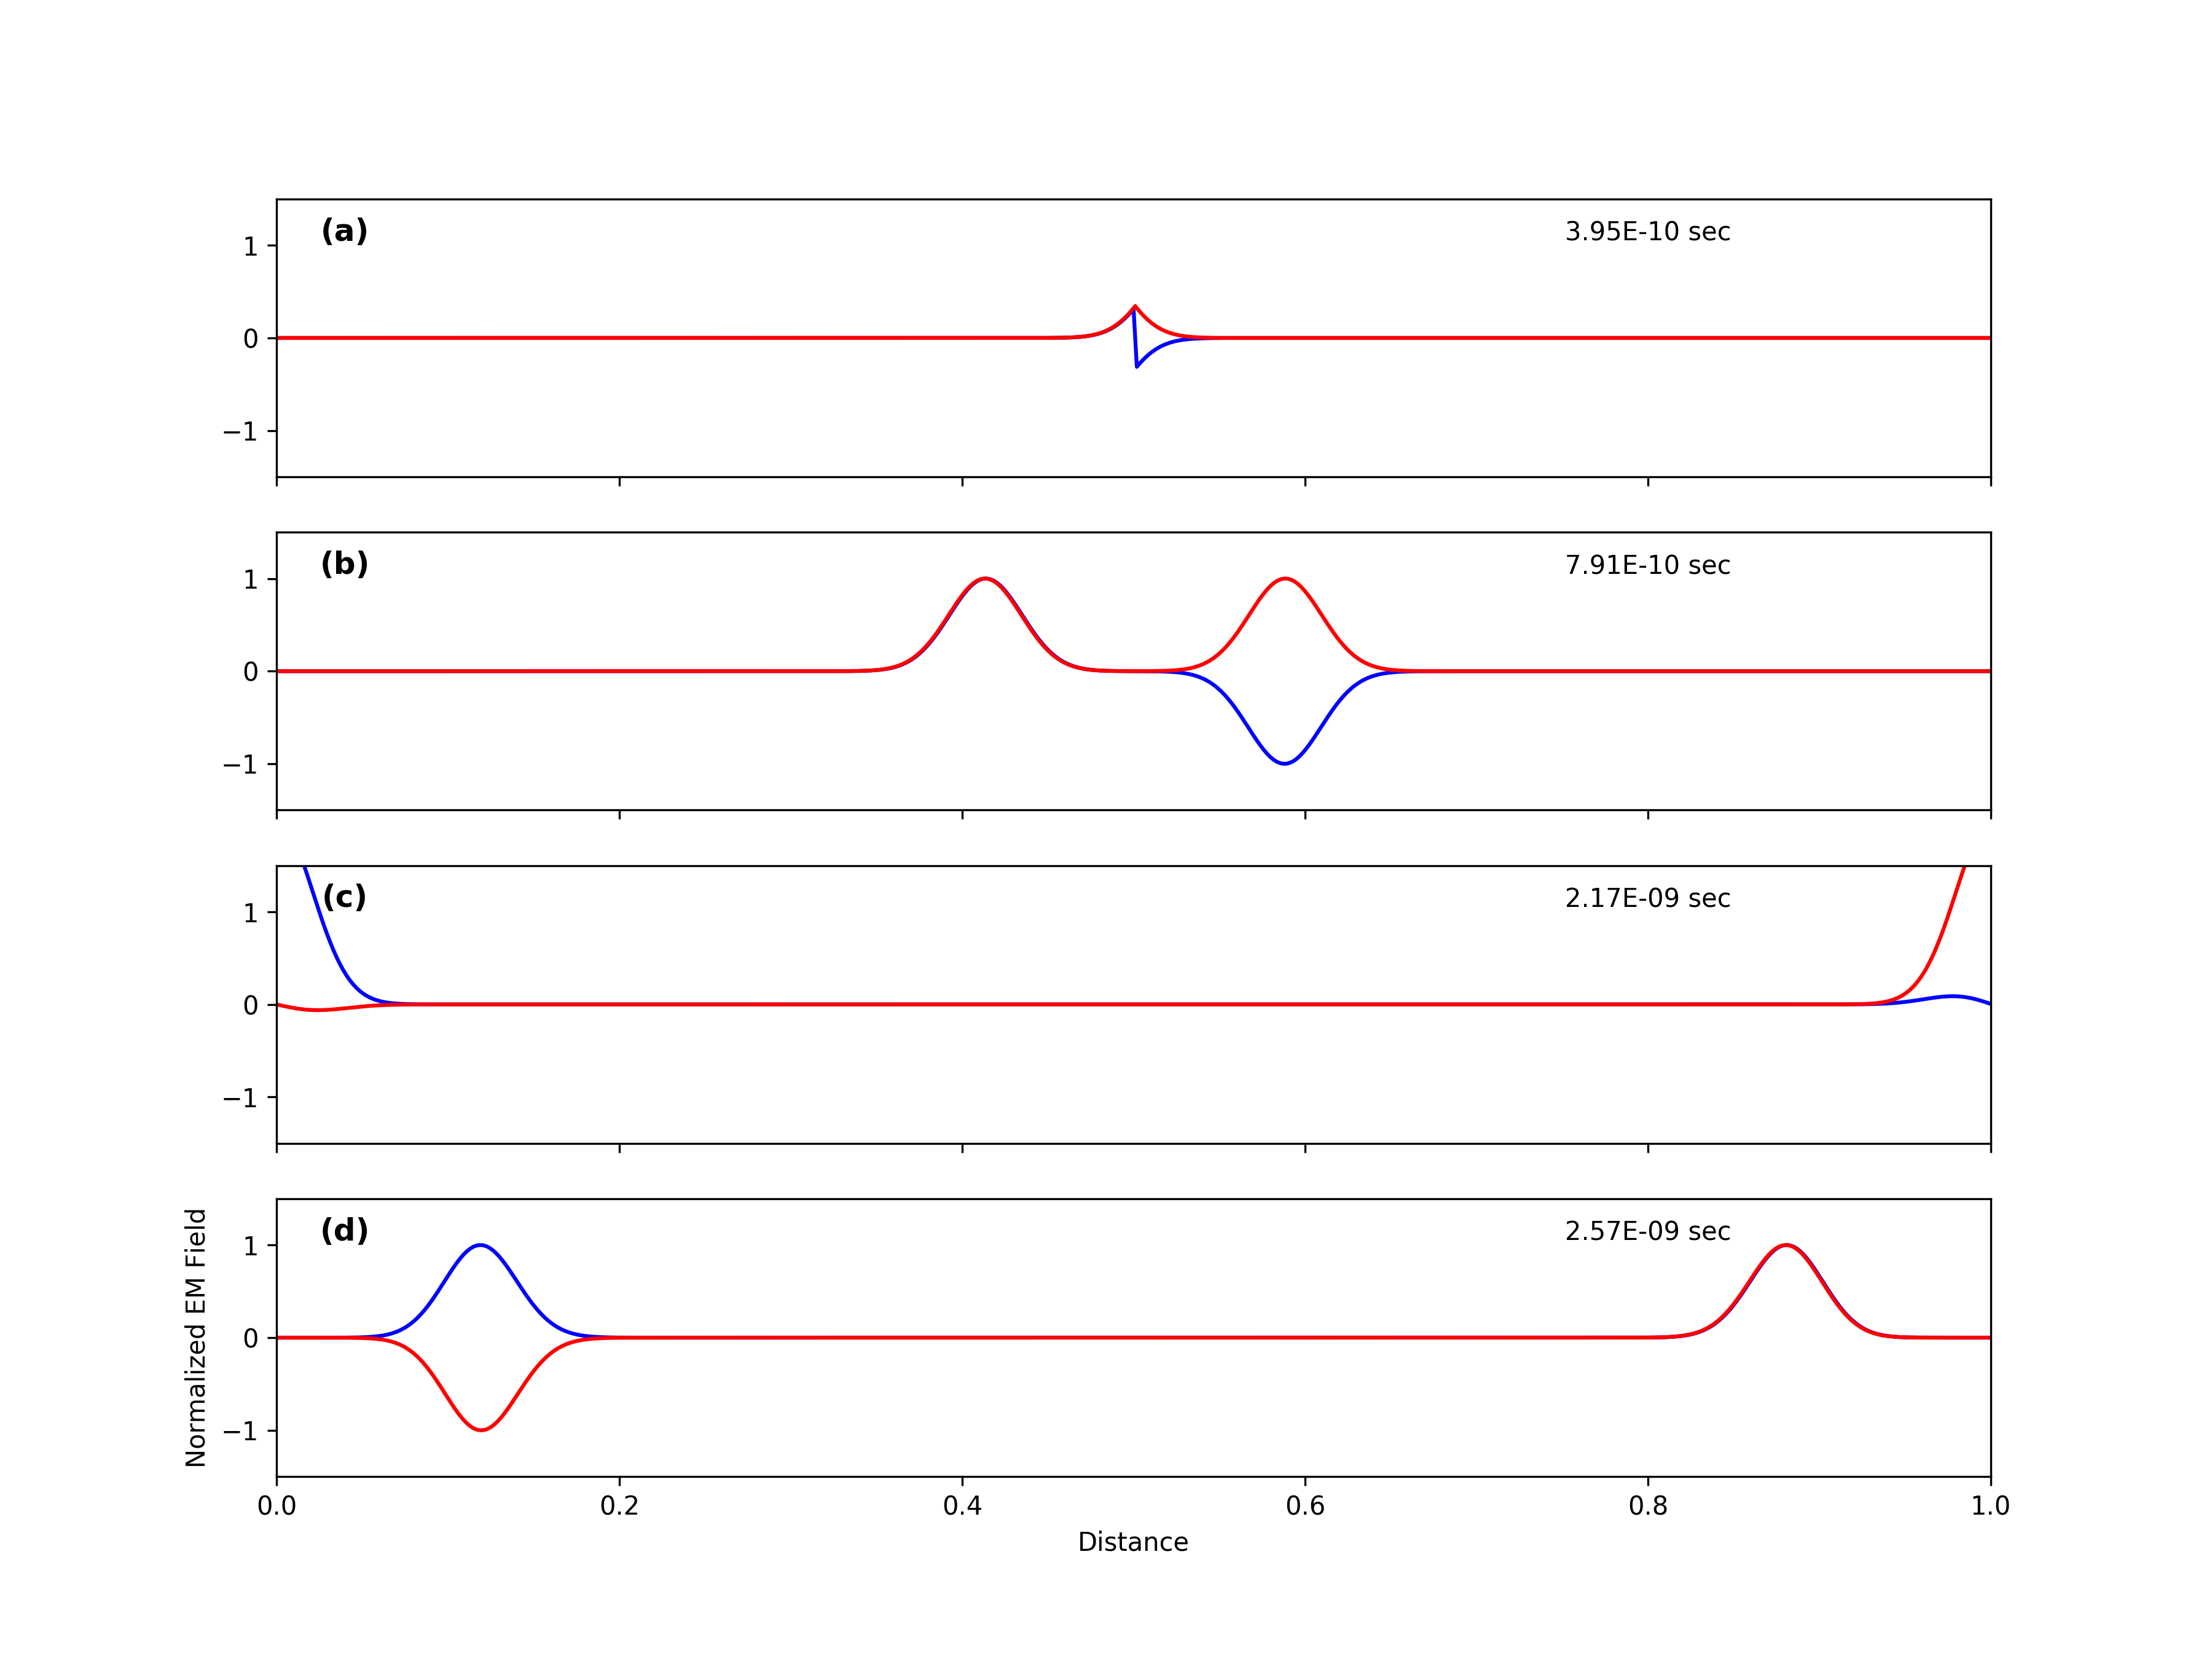
\includegraphics[width=\textwidth]{../DirichletBC.png}
    \caption{A sequence of plots for a one-dimensional finite difference time domain simulation with Dirichlet boundary conditions.}
    \label{fig:YeePML}
\end{figure}


\begin{figure}
    \centering
    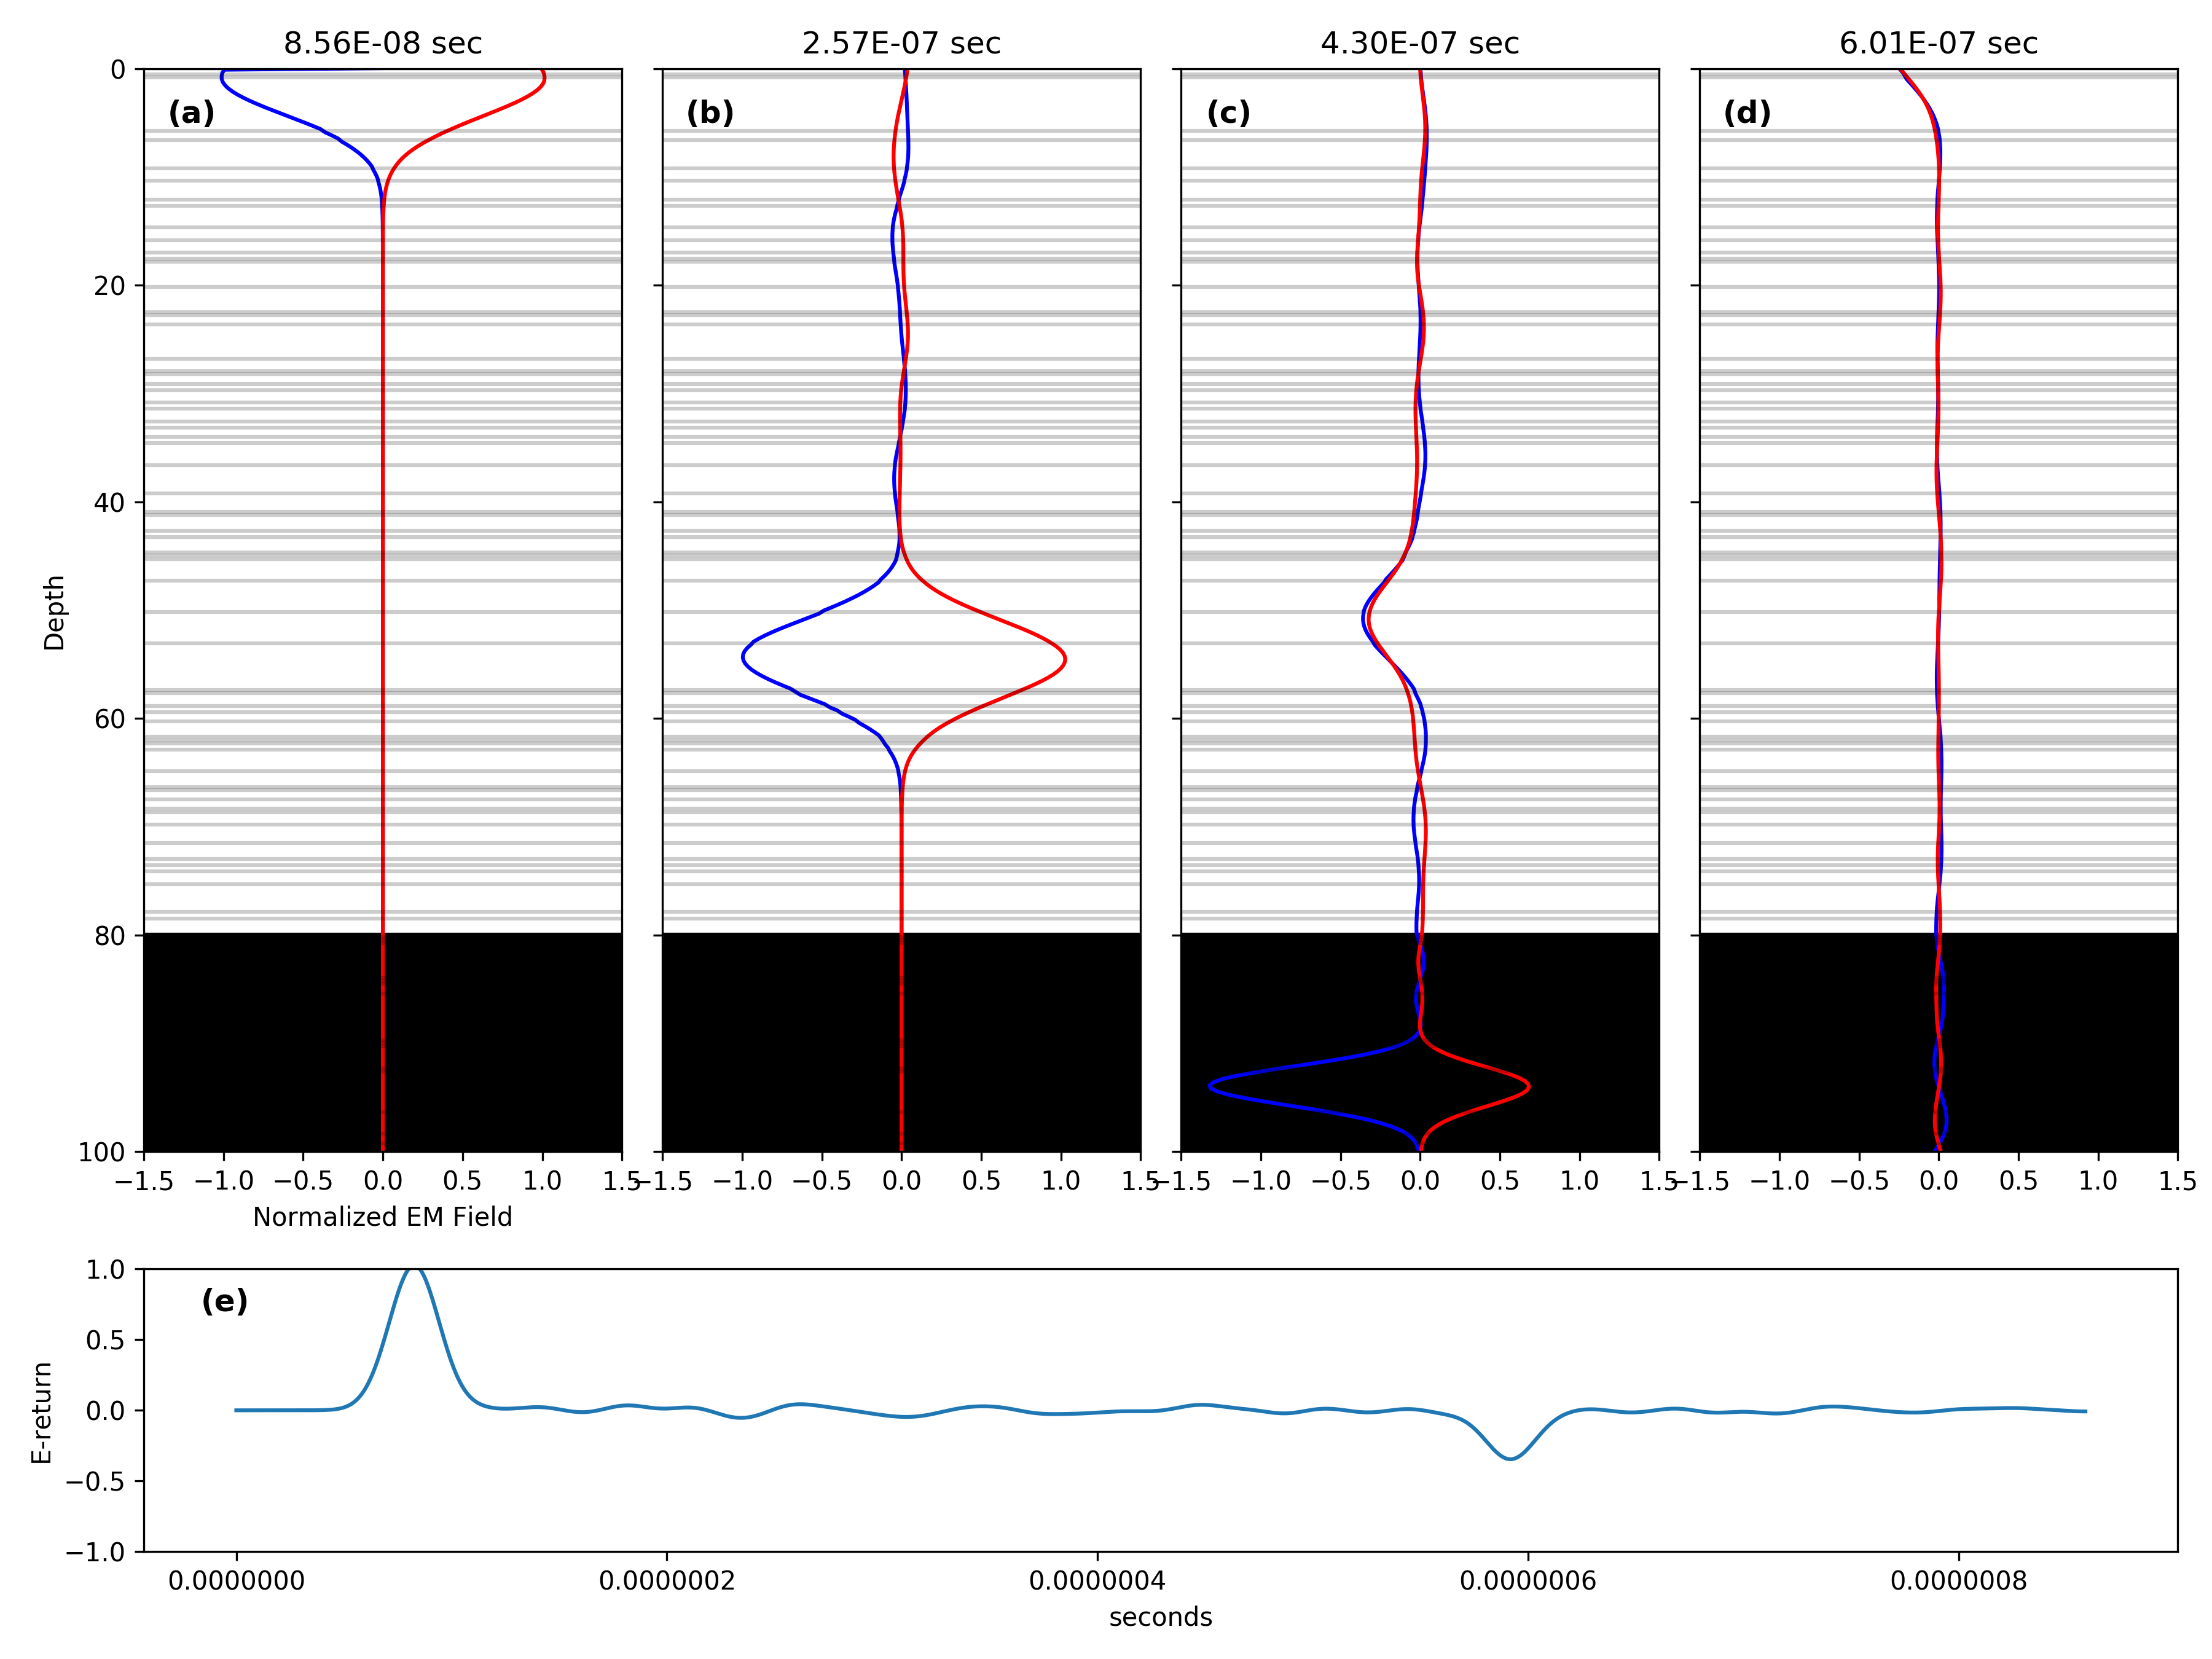
\includegraphics[width=\textwidth]{../IceSimulation.png}
    \caption{Simulation of EM wave propagation through ice.}
    \label{fig:YeePML}
\end{figure}


\begin{figure}
    \centering
    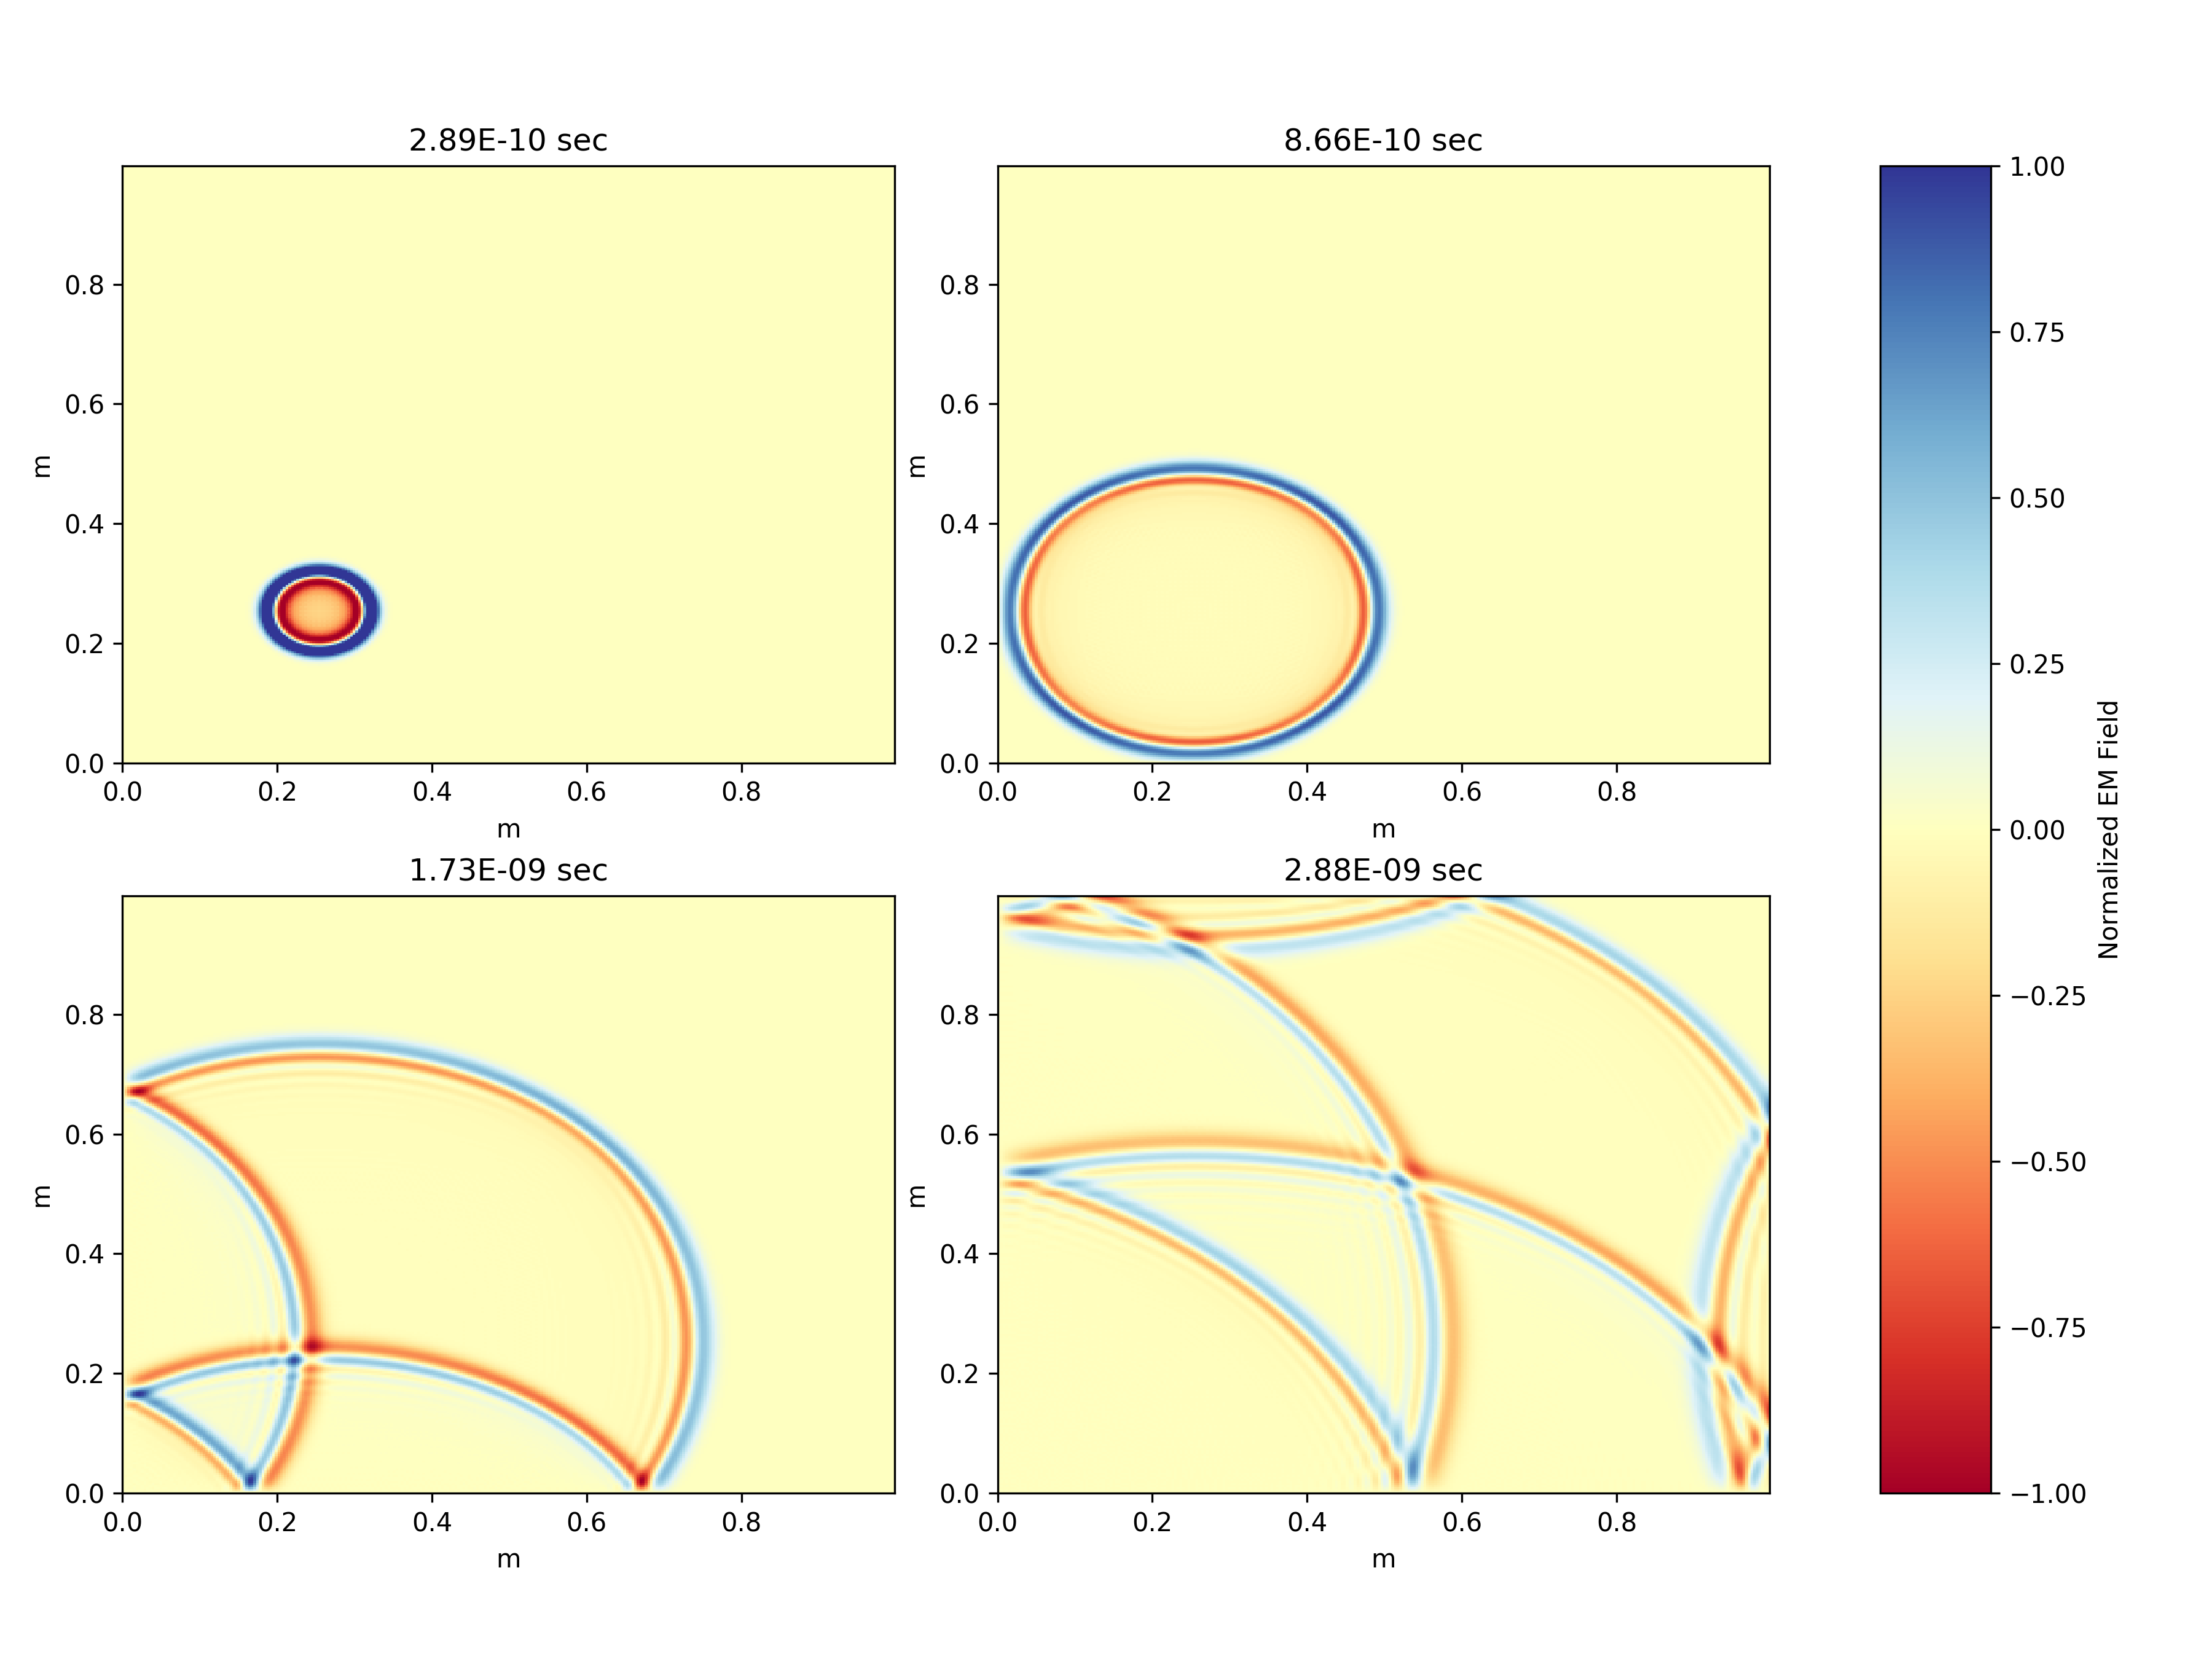
\includegraphics[width=\textwidth]{../2D_figure.png}
    \caption{Two-dimensional finite difference time domain.}
    \label{fig:YeePML}
\end{figure}


\section{Discussion}

\section{Conclusions}

\section*{Data Availability}

Model scripts are available for download as a git repository at \url{https://github.com/benhills/FDTD.git}.

\printbibliography

\end{document}
